\documentclass{article}
\usepackage[a4paper,margin=1.5cm]{geometry}
\usepackage[utf8]{inputenc}

\title{Dynamic labeling}
\author{Elad Noor, Evgeny Onishchenko}

\usepackage{natbib}
\usepackage{graphicx}
\usepackage{amsthm}
\usepackage{amsmath}
\usepackage{amssymb}
\usepackage{mathtools}
\usepackage{hyperref}
\usepackage{pgfplots}

\usepgfplotslibrary{colorbrewer}
\pgfplotsset{cycle list/Set1-8}
\pgfplotsset{compat=1.15}

\newtheorem{theorem}{Theorem}[section]
\newtheorem{corollary}{Corollary}[theorem]
\newtheorem{lemma}[theorem]{Lemma}
\newcommand{\finit}{\ensuremath{\vec{f}^\circ}}
\newcommand{\favg}{\ensuremath{\langle f \rangle}}
\newcommand{\fin}{\ensuremath{\langle f \rangle}}
\newcommand{\stot}{\ensuremath{s_\text{tot}}}
\newcommand{\flux}[2]{\ensuremath{v_{{#1} \rightarrow {#2}}}}

\begin{document}

\maketitle

\section{Introduction}

The internal metabolism of cells has always been a tough nut to crack. Spectroscopic methods that can visualize small molecules cover only a handful of specific compounds. On the other hand, the overlapping spectra of the diverse metabolome of most cells makes it extremely difficult to quantify single metabolites using spectroscopic methods. Therefore, the ubiquitous analytical method used in metabolomic studies is mass spectroscopy (MS), which is both specific and sensitive enough to cover most metabolites in the cell. The downsides are, of course, its destructive nature and the required amounts that currently don't allow for single-cells studies of bacteria.

Another complication that makes metabolism difficult to study, is the inconvenient fact that metabolite abundances are usually not the most important phenotype, but rather metabolic flux. Flux is what directs cell resources through different pathways to the target required for cell proliferation (or other factors that affect fitness). Furthermore, the enzymes required to catalyze metabolic reactions are typically more expensive than the intermediates metabolite pools (in terms of dry weight, ATP requirement, maintenance energy, etc.). This means that evolution does not care as much about metabolite abundance as much as enzyme abundance, and therefore would try to reduce unnecessary fluxes as much as possible. A general strategy in Flux Balance Analysis (FBA) for finding a likely flux solution is to minimize the sum of all fluxes. It is, however, way more difficult to measure fluxes compared to metabolite abundances, since flux is an inherently dynamic property and requires a few assumptions and probing techniques to observe in an essentially static and destructive methods such as MS.

Flux measuring methods can be classified into two main categories: stationary/standard metabolic flux analysis (MFA or stat-MFA) and isotopically non-stationary metabolic flux analysis (abbreviated as INST-MFA \cite{noh_metabolic_2007, jazmin_isotopically_2014}, instat-MFA \cite{heise_flux_2014}, or NMFA\cite{young_elementary_2008, young_inca:_2014}). Both methods introduce a labeled substrate to the media (e.g. $^{13}$C-labeled glucose) and measure the mass isotopomer distributions (MIDs) of certain intracellular metabolites (e.g. amino acids). The main difference is that in standard MFA, measurements are done only after the system has reach isotopic steady state (i.e. the MIDs do not change anymore), while INST-MFA focuses on the transient period right after adding the label to the medium. 

In general, INST-MFA can be used either in metabolic steady-state (where all fluxes and pool sizes are constant) or in perturbed state. Often, the data is used only in a qualitative manner, e.g. to answer which of a set of possible products gets labeled or the timescale required for the labeling to occur. Inferring fluxes from such data is, however, tricky since it also depends on the intermediate metabolite pool sizes and all the inputs and outputs to the pathway. Without the metabolic steady-state assumption, one typically has to simulate the labeling trajectories using a full kinetic model and numeric ODE integration.

Here, we only discuss the case of steady-state labeling. In this case, there is a general solution \cite{young_elementary_2008} which does not require any of the kinetic parameters, only the fluxes and metabolite pool sizes (which are assumed constant). In addition, the ODE system can be solved analytically for some specific cases \cite{sokol_theoretical_2015}, and for all others by simple numerical tools.

\section{General solution for steady state dynamic labeling experiments}
Imagine a general metabolic network, which can be described as a standard graph, i.e. all reactions are one-to-one (typically, metabolic networks for medium size or larger will not qualify here, and it would be necessary to use an atom-mapping network for them).

We assume the system is at metabolic steady state, i.e. therefore all fluxes and pool sizes are constant and given by \flux{i}{j} (the flux from $S_i$ to $S_j$) and $s_i$ (the pool size of $S_i$). Any system with a non-trivial steady-state must be an open system that dissipates free energy, and must have fluxes that exchange material with the ``outside'', also known as \textit{external} fluxes. For the incoming exchange fluxes, we assume that that the they are irreversible or that the outside pools are large enough, so that and that the relatively small fluxes in our system have negligible effect on them. We denote the labeled fractions of these external pools by $h_j$ and the irreversible flux from external pool $j$ to $S_i$ by $y_{j \rightarrow i}$. The number of such pools is $m$. Finally, we will assume that all outgoing exchange fluxes are irreversible as well, and denote the total of all these outgoing fluxes from $S_i$ as $\flux{i}{\emptyset}$.

The labeled fractions of the internal pools ($S_1, \ldots S_n$) are not at steady-state and we aim to describe their time evolution, denoted $f_i(t) \equiv s_i^1(t) / (s_i^0(t) + s_i^1(t)) = s_i^1(t) / s_i$. Note that one $\vec{f}$ and $\vec{y}$ are time dependent in this system, since fluxes and pool sizes are assumed to be at steady-state. Then:
\begin{align}
    s_i \frac{d f_i}{dt} 
    &= \frac{d s_i^0}{dt}
    = \sum_{j=1}^{n} f_j\flux{j}{i} + \sum_{j=1}^m h_j y_{j \rightarrow i} - \sum_{j=1}^n f_i \flux{i}{j} - f_i \flux{i}{\emptyset}\nonumber\\
    &= \sum_{j=1}^{n} f_j\flux{j}{i} + \sum_{j=1}^m h_j y_{j \rightarrow i} - f_i \left( \sum_{j=1}^n \flux{j}{i} + \sum_{j=1}^m y_{j \rightarrow i}\right) \label{eq:steady_state}
\end{align}
where we replaced the sum of all the outgoing fluxes with the sum of all incoming fluxes (they are equal due to the steady-state assumption).

This ODE can also be written also in matrix notation, where we use the convention that ($\vec{\cdot}$) represents a row vector.
\begin{eqnarray}\label{eq:inhom_ode}
	\frac{d\vec{f}}{dt} &=& \vec{f}~\mathbf{M} + \vec{g}
\end{eqnarray}
where $\mathbf{M}$ and $\vec{g}$ are defined as:
\begin{eqnarray}
    \forall i \neq j:& m_{ji} \equiv& \frac{\flux{j}{i}}{s_i} \\
    \forall i:& m_{ii} \equiv& -\frac{1}{s_i} \left(\sum_{j=1}^n \flux{j}{i} + \sum_{j=1}^m y_{j \rightarrow i} \right)\\
    \forall i:& g_{i}(t) \equiv& \frac{1}{s_i} \sum_{j=1}^m h_j(t)~y_{j \rightarrow i}
\end{eqnarray}

\subsection{INST-MFA can be solved as a first order linear inhomogeneous ODE}
The general solution \cite{young_elementary_2008} for the inhomogeneous first order linear ODE in Equation \ref{eq:inhom_ode} is:
\begin{eqnarray}\label{eq:inhom_ode_sol}
    \vec{f}(t) = \vec{f}(0)~e^{\mathbf{M} t} + \int_0^t \vec{g}(\tau) \cdot e^{\mathbf{M} (t-\tau)} d\tau
\end{eqnarray}

In most of this manuscript, we will assume that the internal pools start completely unlabeled, i.e. $\vec{f}(0) = \vec{0}$, and so the term before the integral drops out. In addition, we will focus on the case where there is only one external pool, which turns from unlabeled to fully labeled at time $t = 0$. This means that \[\vec{g} = \begin{bmatrix} y_1 / s_1 & y_2 / s_2 & \ldots & y_n / s_n \end{bmatrix},\] where $y_i$ is the flux from the external pool to $S_i$. Since $\vec{g}$ is now constant, the integral in Equation \ref{eq:inhom_ode_sol} can be solved explicitly:
\begin{eqnarray}
    \vec{f}(t) ~=~ \vec{g} \int_0^t e^{\mathbf{M} (t-\tau)} d\tau ~=~
    \vec{g} ~ \mathbf{M}^{-1} ~ \left( e^{\mathbf{M}t} - \mathbf{I} \right) =
    \vec{g} ~ \mathbf{P} ~ \mathbf{J}^{-1} ~ \left( e^{\mathbf{J}t} - \mathbf{I} \right) \mathbf{P}^{-1}
\end{eqnarray}
where in the last step we used the Jordan normal form, i.e. $\mathbf{M} = \mathbf{P} \mathbf{J} \mathbf{P}^{-1}$.

\subsubsection{Defining the internal average labeled fraction}

We define $\fin$ as the weighted average of labels among all internal pools, namely 
\begin{eqnarray}\label{eq:dfin_dt}
\fin &\equiv& \frac{\sum_{i=1}^{n} f_i \, s_i}{\sum_{i=1}^{n} s_i}
\end{eqnarray}

$\fin$ is useful in some experimental setups, where the internal average labeled fraction can be directly measured. For instance, the $^{13}$C fraction of all biomass carbons can be measured by complete oxidation of dry biomass to carbon dioxide (after removing all the externally labeled compounds in the media by separating the supernatant).

To find a description for $\fin$ as a function of time, we first calculate the time derivative:
\begin{eqnarray}
\frac{d\fin}{dt} &=& \frac{\sum_{i=1}^{n} s_i~\frac{d f_i}{dt}}{\sum_{i=1}^{n} s_i} \,.
\end{eqnarray}

Comparing to Equation \ref{eq:steady_state}, we see that the numerator is given by its sum over $i$:
\begin{eqnarray}
    \sum_{i=1}^{n} s_i~\frac{d f_i}{dt} &=& \sum_{i=1}^n \left(\sum_{j=1}^{n} f_j\flux{j}{i} + \sum_{j=1}^m h_j y_{j \rightarrow i} - \sum_{j=1}^n f_i \flux{i}{j} - f_i \flux{i}{\emptyset}\right) \\
    &=& \sum_{i,j} f_j\flux{j}{i} - \sum_{i,j} f_i\flux{i}{j} + 
    \sum_{i=1}^n \sum_{j=1}^m h_j y_{j \rightarrow i} - \sum_{i=1}^n f_i \flux{i}{\emptyset}
\end{eqnarray}
where we note that the first two sums cancel each other out. Therefore, the simplified expression for the time derivative of the average labeled fractions is:
\begin{eqnarray}
    \frac{d\fin}{dt} &=& \frac{\sum_{i=1}^n \sum_{j=1}^m h_j y_{j \rightarrow i} - \sum_{i=1}^n f_i \flux{i}{\emptyset}}{\sum_{i=1}^{n} s_i}\,.
\end{eqnarray}

This equation also makes logical sense, since if we consider all internal pools as one big pool, the left term of the numerator represents the total amount of label coming into it per time, and the right term is the label leaving the system. The denominator is the total internal pool size.

\subsection{Example: linear pathway with only irreversible steps}
Imagine a cascade of reactions which is at steady state, but the fluxes are not necessarily equal (e.g. there could be irreversible branching fluxes):
\begin{equation}
    \xrightarrow{v_1} \underset{\downarrow}{S_1} 
    \xrightarrow{v_2} \underset{\downarrow}{S_2}
    \xrightarrow{v_3} \ldots 
    \xrightarrow{v_n} \underset{\downarrow}{S_n}
\end{equation}
We define $\tau_i \equiv \frac{s_i}{v_i}$ in order to reduce the number of parameters. The system is therefore described by:
\begin{eqnarray}
\mathbf{M} =
  \begin{bmatrix}
    -1/\tau_1 & 1/\tau_2 & 0 & \ldots & 0 & 0\\
    0 & -1/\tau_2 & 1/\tau_3 & \ldots & 0 & 0\\
    0 & 0 & -1/\tau_3 & \ldots & 0 & 0\\
    \vdots\\
    0 & 0 & 0 & \ldots & 0 & -1/\tau_n
  \end{bmatrix}
~~~~~
\vec{g} = \left[1/\tau_1~0~0~\ldots~0\right]\,.
\end{eqnarray}

We note that as $\mathbf{M}$ is triangular, its Jordan normal form is a diagonal matrix. Therefore, we can write $\mathbf{M} = \mathbf{P} \mathbf{D} \mathbf{P}^{-1}$, where $\mathbf{D}$ has the same values as the diagonal values of $\mathbf{M}$ (assuming they are distinct -- we discuss other cases in the next section). To simplify the solution for this ODE system, we define $\forall i \neq j:~q_{ij} \equiv (1 - \tau_i/\tau_j)^{-1}$, and $\forall i:~q_{ii} \equiv 1$, and use \href{https://www.sympy.org/}{Sympy} to find the Jordam normal form and calculate:
\[
\mathbf{P}^{-1} =
\begin{bmatrix}
1 & \prod_{2}^2 q_{i1} & \prod_{2}^3 q_{i1} & \ldots & \prod_{2}^n q_{i1} \\
0 & 1 & \prod_{3}^3 q_{i2} & \ldots & \prod_{3}^n q_{i2} \\
0 & 0 & 1 & \ldots & \prod_{4}^n q_{i3} \\
\vdots\\
0 & 0 & 0 & \ldots & 1
\end{bmatrix}
\]
and:
\[
    \vec{g}~\mathbf{P}~\mathbf{J}^{-1}~\left( e^{\mathbf{J} t} - \mathbf{I} \right)
    =
    \begin{bmatrix}
        (1 - e^{-t/\tau_1})\prod_{1}^1 q_{i1} & (e^{-t/\tau_2}-1) \prod_{1}^2 q_{i2} & \ldots & (e^{-t/\tau_n}-1) \prod_{1}^n q_{in}
    \end{bmatrix}.
\]

Using these results in Equation \ref{eq:inhom_ode_sol} yields the following expression (where we move the $q$ products from the vector to the matrix on the right):
\begin{eqnarray}
	\vec{f}(t) ~=~
    \begin{bmatrix}
        1 - e^{-t/\tau_1} & e^{-t/\tau_2}-1 & \ldots & e^{-t/\tau_n}-1
    \end{bmatrix}
    \begin{bmatrix}
        \prod_1^1 q_{i1} & \prod_1^2 q_{i1} & \prod_1^3 q_{i1}  & \ldots & \prod_1^n q_{i1} \\ \\
        0 & \prod_1^2 q_{i2} & \prod_1^3 q_{i2} & \ldots & \prod_1^n q_{i2} \\
        \vdots\\
        0 & 0 & 0 & \ldots & \prod_1^n q_{in}
    \end{bmatrix}\label{eq:lin_path_solution}
\end{eqnarray}

We can also write this equation in a compact way without using matrix multiplications:
\begin{eqnarray}
f_i(t) &=& 
    \left(\prod_{k=1}^i q_{k1}\right) (1 - e^{-t/\tau_1}) ~+~
    \sum_{j=2}^i \left(\prod_{k=1}^i q_{kj}\right) (e^{-t/\tau_j} - 1)
\end{eqnarray}

\subsection{Non-distinct eigenvalues}\label{sec:equal_taus}
For our general solution in Equation \ref{eq:lin_path_solution}, we made an important implicit assumption, that none of the $\tau_i$ are equal. If there exist $i \neq j$ where $\tau_i = \tau_j$, then the Jordan normal form would not be a diagonal matrix (and also we would get that $g_{ij} = \infty$). Solving all such cases analytically for an arbitrarily large system is not possible. We can, however, solve the most simple case where and $\tau_1 = \tau_2 = \ldots = \tau_n = \tau$. I similar derivation can also be found in \cite{sokol_theoretical_2015}.

\begin{eqnarray}
\mathbf{M} =
\begin{bmatrix}
-1/\tau & 1/\tau & 0 & \ldots & 0 & 0\\
0 & -1/\tau & 1/\tau & \ldots & 0 & 0\\
\vdots\\
0 & 0 & 0 & \ldots & -1/\tau & 1/\tau\\
0 & 0 & 0 & \ldots & 0 & -1/\tau \\
\end{bmatrix}
~~~~~
\vec{g} = \left[1/\tau~0~0~\ldots~0\right]\,.
\end{eqnarray}

In this case, $\mathbf{J}$ is not a diagonal matrix, which makes the matrix solution seem a bit more complicated. However, SymPy can directly solve the equation, which is turns out to be:
\begin{eqnarray}\label{eq:equal_tau_solution}
    f_i(t) = 1 - e^{-\frac{t}{\tau}}\sum_{k=0}^{i-1} \frac{1}{k!}\left(\frac{t}{\tau}\right)^k\,.
\end{eqnarray}

\section{Linear irreversible pathway with dilution}\label{sec:linear_examples}
Assume that the pathway exists inside an exponentially growing cell, all species are at steady state, and that no side fluxes exist besides the growth dilution (which is given by $\flux{i}{\emptyset} = \mu s_i$). In addition, the final product $S_n$ is a dead-end (e.g. it could be a direct constituent of biomass like a membrane lipid). The fluxes are thus given by:
\begin{equation}
    \flux{i-1}{i} = \mu \sum_{k=i}^n s_k
\end{equation}
and therefore $\tau_i = s_i/v_i = s_i (\mu \sum_{k=i}^n s_k)^{-1}$. It is convenient to define the relative pool size of $S_i$ compared to all the downstream pool (including $S_i$ itself) as $\phi_i \equiv \mu\tau_i = s_i / \sum_{k=i}^n s_k$. In this case:
\begin{equation}\label{eq:dilution}
    f_i(t) = 1 - \sum_{j=1}^{i} \left(\prod_{k = 1, i \neq j}^{i} 1 - \phi_k/\phi_j\right)^{-1} e^{- \mu t / \phi_j}
\end{equation}

There is only one input flux, going into $S_1$, i.e. $y_{1 \rightarrow 1} = \mu \sum s_i$. We assume it is fully labeled, so $h_1 = 1$. We can now calculate $\fin$ as a function of time, by plugging these values into Equation \ref{eq:dfin_dt}:
\begin{eqnarray}
	\frac{d\fin}{dt}
	= 
	\frac{\sum_{i=1}^n \sum_{j=1}^m h_j y_{j \rightarrow i} - \sum_{i=1}^n f_i \flux{i}{\emptyset}}{\sum_{i=1}^{n} s_i} 
	=
	\frac{\mu \sum_{i=1}^{n} s_i - \sum_{i=1}^{n} f_i \mu s_i }{\sum_{i=1}^{n} s_i}
	=
	\mu \frac{\sum_{i=1}^{n} s_i - \sum_{i=1}^{n} f_i s_i }{\sum_{i=1}^{n} s_i}
	=
    \mu \left(1 - \fin\right)
\end{eqnarray}
Since $\fin(0) = 0$, the solution is:
\begin{eqnarray}
	\fin = 1 - e^{-\mu\,t} \label{eq:fin_dilution}
\end{eqnarray}


\subsection{Example: four equal pool sizes}
In this example, we choose $n = 4$, $\mu = 1$ hour$^{-1}$ and $s_1 = \ldots = s_4$. Then $\phi_i = 1/(5-i)$ and therefore:
\begin{center}
\begin{tabular}{cccccc}
    $f_1$ = & 1 & $- e^{-4t}$ &&&\\
    $f_2$ = & 1 & $+ 3 e^{-4t}$ & $- 4 e^{-3t}$ &&\\
    $f_3$ = & 1 & $+ 3 e^{-4t}$ & $+ 8 e^{-3t}$ & $- 6 e^{-2t}$ &\\
    $f_4$ = & 1 & $- e^{-4t}$   & $- 4 e^{-3t}$ & $+ 6 e^{-2t}$ & $- 4 e^{-t}$
\end{tabular}
\end{center}

We can see that our solution for $\fin$ (Equation \ref{eq:fin_dilution}) is indeed correct by calculating it explicitly:
\begin{equation}
    \fin = \frac{s_1 f_1 + s_2 f_2 + s_3 f_3 + s_4 f_4}{s_1 + s_2 + s_3 + s_4} = \frac{f_1 + f_2 + f_3 + f_4}{4} = 1 - e^{-t}
\end{equation}

We can now visualize all four fractions and the average $\fin$:
\begin{center}
	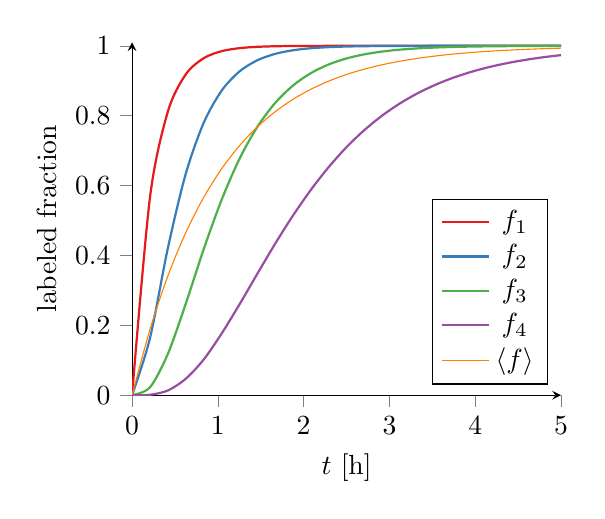
\begin{tikzpicture}
	\begin{axis}[width=200pt,axis x line=bottom, axis y line=left, tick align=outside, domain=0:5, xlabel={$t$ [h]}, ylabel={labeled fraction}, ymin=0, ymax=1.01, legend pos=south east]
    	\addplot+[mark=none,smooth,thick] (\x,{ 1 - exp(-4*\x) });
    	\addlegendentry{$f_1$}
    	\addplot+[mark=none,smooth,thick] (\x,{ 1 + 3*exp(-4*\x) - 4*exp(-3*\x) });
    	\addlegendentry{$f_2$}
    	\addplot+[mark=none,smooth,thick] (\x,{ 1 - 3*exp(-4*\x) + 8*exp(-3*\x) - 6*exp(-2*\x) });
    	\addlegendentry{$f_3$}
    	\addplot+[mark=none,smooth,thick] (\x,{ 1 + 1*exp(-4*\x) - 4*exp(-3*\x) + 6*exp(-2*\x) - 4*exp(-\x) });
    	\addlegendentry{$f_4$}
    	\addplot+[mark=none,smooth] (\x,{ 1 - exp(-\x) });
    	\addlegendentry{$\fin$}
    \end{axis}
	\end{tikzpicture}
\end{center}

\subsection{2-step assembly process with unknown pool sizes}
Here, we consider the most simple case of protein complex assembly. We assume that we can measure the labeling of the prey protein before and after forming a complex with the bait, denoted \textit{precursor pool} and \textit{bound pool} with the corresponding pool sizes ($s_1$ and $s_2$). As before, at time $t = 0$, any newly synthesized protein would be labeled. Additionally, we assume no degradation and irreversible binding. The only diluting factor is the growth rate $\mu$.

So, we can use the general solution from equation \ref{eq:dilution}, where $\phi_1 = s_1 / (s_1 + s_2)$ and $\phi_2 = 1$:
\begin{eqnarray}
    f_1 &=& 1 - e^{- \mu t / \phi_1} \\
    f_2 &=& 1 - \left(1 - 1 / \phi_1 \right)^{-1} e^{- \mu t / \phi_1} - \left(1 - \phi_1 \right)^{-1} e^{- \mu t}
\end{eqnarray}
To We can now rewrite $f_2$ as a function of $f_1$ and thus get rid of $t$:
\begin{eqnarray}
    f_2 &=& 1 + \frac{\phi_1}{1-\phi_1} (1 - f_1) - \frac{1}{1-\phi_1} (1 - f_1)^{\phi_1}
\end{eqnarray}
which is a function that looks like this:
\begin{center}
	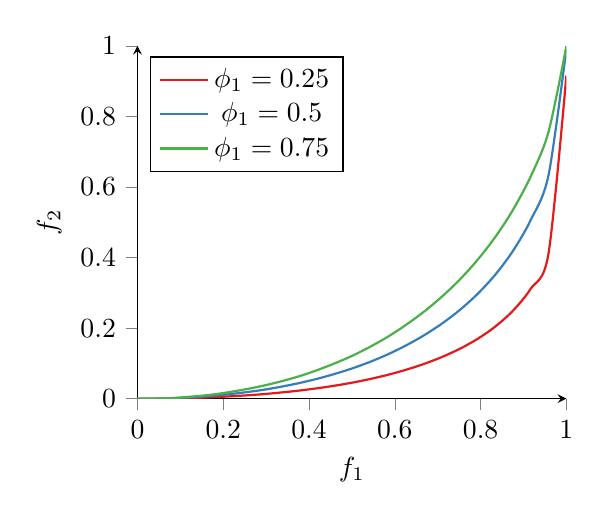
\begin{tikzpicture}[
		declare function={ f2(\x,\y) = 1 + \y/(1-\y)*(1-\x) - 1/(1-\y)*(1-x)^\y ;
		},
	]
	\begin{axis}[width=200pt,axis x line=bottom, axis y line=left, tick align=outside, domain=0:1, xmin=0, xmax=1, xlabel={$f_1$}, ylabel={$f_2$}, ymin=0, ymax=1, legend pos=north west]
    	\addplot+[mark=none,smooth,thick] (\x,{ f2(\x, 0.25) });
    	\addlegendentry{$\phi_1 = 0.25$}
    	\addplot+[mark=none,smooth,thick] (\x,{ f2(\x, 0.5) });
    	\addlegendentry{$\phi_1 = 0.5$}
    	\addplot+[mark=none,smooth,thick] (\x,{ f2(\x, 0.75) });
    	\addlegendentry{$\phi_1 = 0.75$}
	\end{axis}
	\end{tikzpicture}
\end{center}

We can also rewrite the two fraction $f_1$ and $f_2$ as functions of $\fin = 1 - e^{- \mu t}$:
\begin{eqnarray}
    f_1 &=& 1 - (1 - \fin)^{1/{\phi_1}} \label{eq:two_step_f1_vs_ftot} \nonumber\\
    f_2 &=& 1 + \frac{\phi_1}{1-\phi_1} (1 - \fin)^{1/{\phi_1}} - \frac{1}{1-\phi_1} (1 - \fin) \label{eq:two_step_f2_vs_ftot}
\end{eqnarray}

\begin{center}
	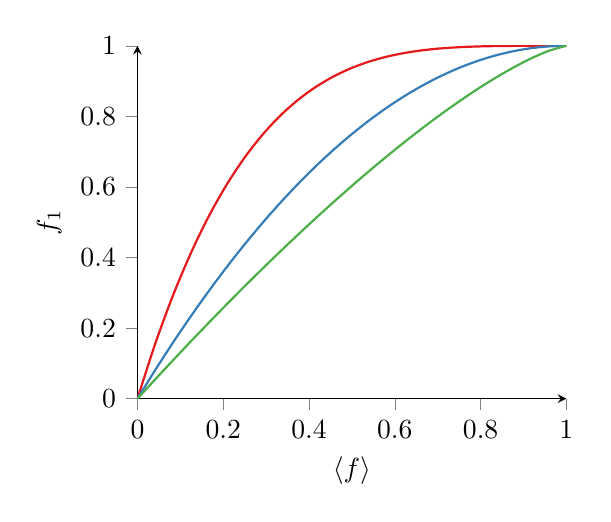
\begin{tikzpicture}[
		declare function={ f1(\x,\y) = 1-(1-\x)^(1/\y) ;
		},
	]
	\begin{axis}[width=200pt,axis x line=bottom, axis y line=left, tick align=outside, domain=0:1, xmin=0, xmax=1, xlabel={$\fin$}, ylabel={$f_1$}, ymin=0, ymax=1, legend pos=south east]
    	\addplot+[mark=none,smooth,thick] (\x,{ f1(\x, 0.25) });
    	\addplot+[mark=none,smooth,thick] (\x,{ f1(\x, 0.5) });
    	\addplot+[mark=none,smooth,thick] (\x,{ f1(\x, 0.75) });
	\end{axis}
	\end{tikzpicture}
	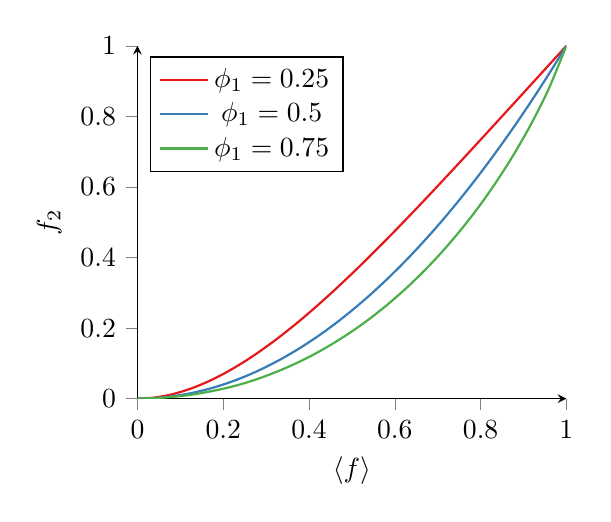
\begin{tikzpicture}[
		declare function={ f2(\x,\y) = 1 + \y/(1-\y)*(1-\x)^(1/\y) - 1/(1-\y)*(1-\x) ;
		},
	]
	\begin{axis}[width=200pt,axis x line=bottom, axis y line=left, tick align=outside, domain=0:1, xmin=0, xmax=1, xlabel={$\fin$}, ylabel={$f_2$}, ymin=0, ymax=1, legend pos=north west]
    	\addplot+[mark=none,smooth,thick] (\x,{ f2(\x, 0.25) });
    	\addlegendentry{$\phi_1 = 0.25$}
    	\addplot+[mark=none,smooth,thick] (\x,{ f2(\x, 0.5) });
    	\addlegendentry{$\phi_1 = 0.5$}
    	\addplot+[mark=none,smooth,thick] (\x,{ f2(\x, 0.75) });
    	\addlegendentry{$\phi_1 = 0.75$}
	\end{axis}
	\end{tikzpicture}
\end{center}

If measuring both $f_1$ and $\fin$ is possible, there is an analytical solution for $\phi_1$:
\begin{eqnarray}
    \phi_1 &=& \frac{\ln(1-\fin)}{\ln(1-f_{1})}
\end{eqnarray}
but unfortunately, we can typically only measure $f_2$ and $\fin$, so solving for $\phi_1$ must be done numerically.

\begin{center}
	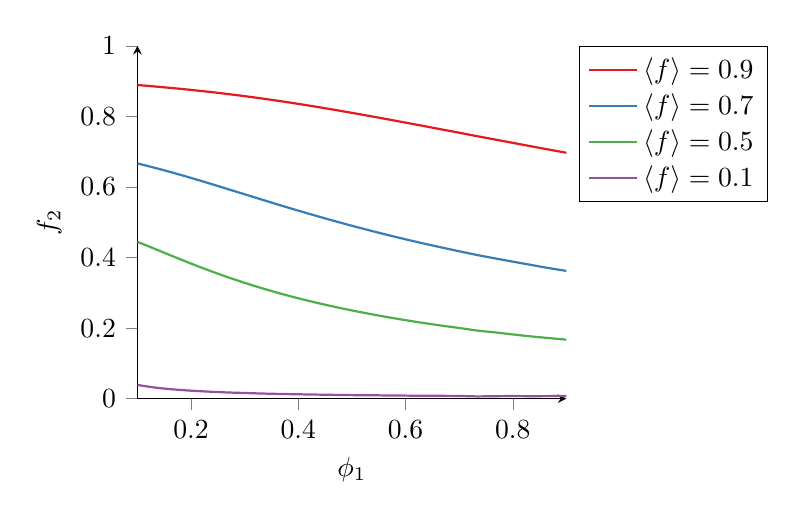
\begin{tikzpicture}[
		declare function={ f2(\x,\y) = 1+\x/(1-\x)*(1-\y)^(1/\x) - 1/(1-\x)*(1-\y);
		},
	]
    \begin{axis}[width=200pt,axis x line=bottom, axis y line=left, tick align=outside, domain=0.1:0.9, xlabel={$\phi_1$}, ylabel={$f_2$}, ymin=0, ymax=1, legend pos=outer north east]
    	\addplot+[mark=none,smooth,thick] (\x,{ f2(\x, 0.9) });
    	\addlegendentry{$\fin = 0.9$}
    	\addplot+[mark=none,smooth,thick] (\x,{ f2(\x, 0.7) });
    	\addlegendentry{$\fin = 0.7$}
    	\addplot+[mark=none,smooth,thick] (\x,{ f2(\x, 0.5) });
    	\addlegendentry{$\fin = 0.5$}
    	\addplot+[mark=none,smooth,thick] (\x,{ f2(\x, 0.1) });
    	\addlegendentry{$\fin = 0.1$}
	\end{axis}
	\end{tikzpicture}
\end{center}


\subsection{3-step assembly process with unknown pool sizes}
Another common case we consider, is similar to the 2-step assembly, except that bound proteins can continue on to an \textit{inaccessible pool} with an unknown size.

So, we can use the general solution from equation \ref{eq:dilution}, where $\phi_1 = s_1 / (s_1 + s_2 + s_3)$, $\phi_2 = s_2 / (s_2 + s_3)$ and $\phi_3 = 1$:
\begin{eqnarray}
    f_1 &=& 1 - e^{- \mu t / \phi_1} \nonumber\\
    f_2 &=& 1 - \left(1 - \phi_2 / \phi_1 \right)^{-1} e^{- \mu t / \phi_1} - \left(1 - \phi_1 / \phi_2 \right)^{-1} e^{- \mu t / \phi_2} \nonumber\\
    f_3 &=& 1 - \left(1 - \phi_2 / \phi_1 \right)^{-1} \left(1 - \phi_3 / \phi_1 \right)^{-1} e^{- \mu t / \phi_1} - \left(1 - \phi_1 / \phi_2 \right)^{-1} \left(1 - \phi_3 / \phi_2 \right)^{-1} e^{- \mu t / \phi_2} - \nonumber\\
    && \left(1 - \phi_1 / \phi_3 \right)^{-1} \left(1 - \phi_2 / \phi_3 \right)^{-1} e^{- \mu t / \phi_3}
\end{eqnarray}

As before, we only care about $f_2$ and $\fin$ since they are measurable, so we express one as a function of the other:
\begin{eqnarray}
    \fin &=& 1 - e^{- \mu t}\nonumber\\
    f_2 &=& 1 + \frac{\phi_1}{\phi_2 - \phi_1} (1 - \fin)^{1/{\phi_1}} - \frac{\phi_2}{\phi_2-\phi_1} (1 - \fin)^{1/{\phi_2}} \label{eq:three_step_f2}
\end{eqnarray}

Importantly, there is a complete symmetry between $\phi_1$ and $\phi_2$ (i.e. $f_2(\phi_1, \phi_2) = f_2(\phi_2, \phi_1)$, and that means that if we use this function to fit experimental data, we would not be able to distinguish between two equivalent solutions ($\phi_1$, $\phi_2$) and ($\phi_2$, $\phi_1$).

The effect of a large inaccessible pool (small $\phi_2$) is to shift the curves to the left (i.e. make the labeling of $f_2$ occur at earlier and at lower levels of $\fin$), as seen in the following example:
\begin{center}
	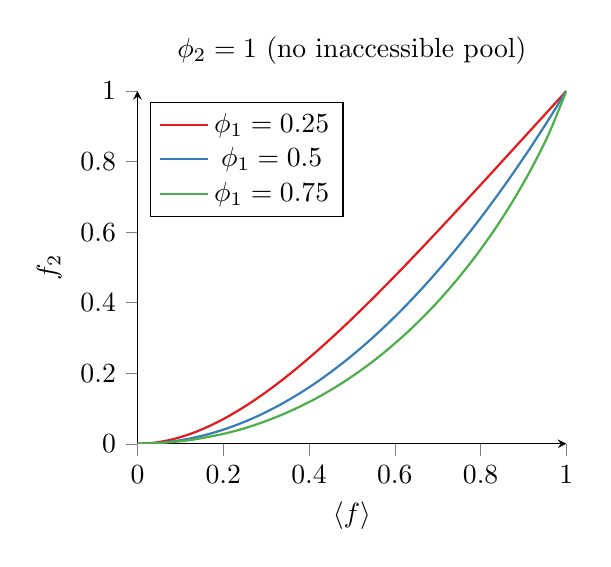
\begin{tikzpicture}[
		declare function={ f2(\x,\y,\z) = 1 + \y/(\z - \y)*(1-\x)^(1/\y) - \z/(\z - \y)*(1-\x)^(1/\z);
		},
	]
	\begin{axis}[title={$\phi_2 = 1$ (no inaccessible pool)}, width=200pt,axis x line=bottom, axis y line=left, tick align=outside, domain=0:1, xlabel={$\fin$}, ylabel={$f_2$}, ymin=0, ymax=1, legend pos=north west]
    	\addplot+[mark=none,smooth,thick] (\x,{ f2(\x, 0.25, 1) });
		\addlegendentry{$\phi_1 = 0.25$}
		\addplot+[mark=none,smooth,thick] (\x,{ f2(\x, 0.5, 1) });
		\addlegendentry{$\phi_1 = 0.5$}
		\addplot+[mark=none,smooth,thick] (\x,{ f2(\x, 0.75, 1) });
		\addlegendentry{$\phi_1 = 0.75$}
	\end{axis}
	\end{tikzpicture}
	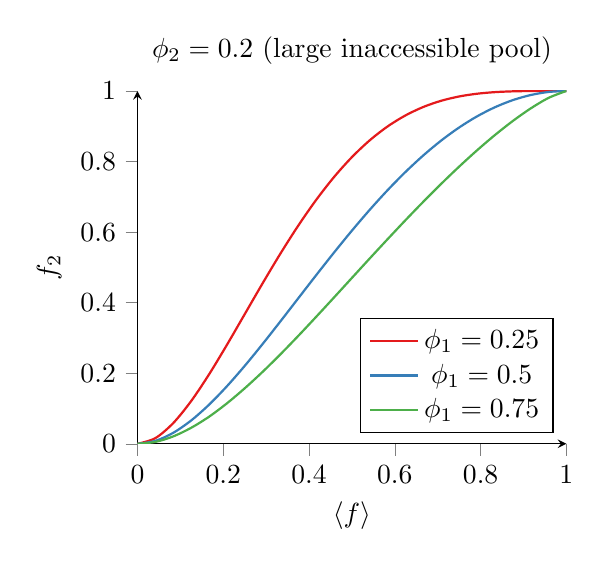
\begin{tikzpicture}[
		declare function={ f2(\x,\y,\z) = 1 + \y/(\z - \y)*(1-\x)^(1/\y) - \z/(\z - \y)*(1-\x)^(1/\z);
		},
	]
	\begin{axis}[title={$\phi_2 = 0.2$ (large inaccessible pool)}, width=200pt,axis x line=bottom, axis y line=left, tick align=outside, domain=0:1, xlabel={$\fin$}, ylabel={$f_2$}, ymin=0, ymax=1, legend pos=south east]
    	\addplot+[mark=none,smooth,thick] (\x,{ f2(\x, 0.25, 0.2) });
		\addlegendentry{$\phi_1 = 0.25$}
    	\addplot+[mark=none,smooth,thick] (\x,{ f2(\x, 0.5, 0.2) });
    	\addlegendentry{$\phi_1 = 0.5$}
    	\addplot+[mark=none,smooth,thick] (\x,{ f2(\x, 0.75, 0.2) });
    	\addlegendentry{$\phi_1 = 0.75$}
	\end{axis}
	\end{tikzpicture}
\end{center}
As expected, the figure on the left ($\phi_2 = 1$) is identical to the one in the previous section (2-step model). We can conclude that $f_2$ decreases with $\phi_1$ as well as $\phi_2$.

\subsection{Solution for the limit of equal \texorpdfstring{$\phi$}{phi} values}
The function in equation \ref{eq:three_step_f2} is not defined for $\phi_1 = \phi_2$ (since we have a 0 divided by 0 situation). However, we can solve the limit using L'H\^{o}pital's rule (we assume $\phi_1$ is constant and derive the numerator and denominator according to $\phi_2$):
\begin{eqnarray}
	f_2 &=& 
	\frac{\phi_2 - \phi_1 + \phi_1 (1-\fin)^{1/{\phi_1}} - \phi_2 (1-\fin)^{1/{\phi_2}}}{\phi_2 - \phi_1}
	\nonumber\\
	&=& \frac{1 - (1-\fin)^{1/{\phi_2}} + \phi_2 \cdot \phi_2^{-2} \cdot \ln{(1-\fin)} \cdot(1-\fin)^{1/{\phi_2}}}{1}
	\nonumber\\
	&=& 1 - \left(1 - \frac{\ln{(1-\fin)}}{\phi_2} \right) \cdot (1-\fin)^{1/{\phi_2}} \label{eq:equal_phi_solution}
\end{eqnarray}
where we used the formula $\frac{\partial a^{f(x)}}{\partial x} = \frac{\partial f}{\partial x}\ln(a) a^{f(x)}$. This is what this function looks like for several values of $\phi_1 = \phi_2 = \phi$:
\begin{center}
	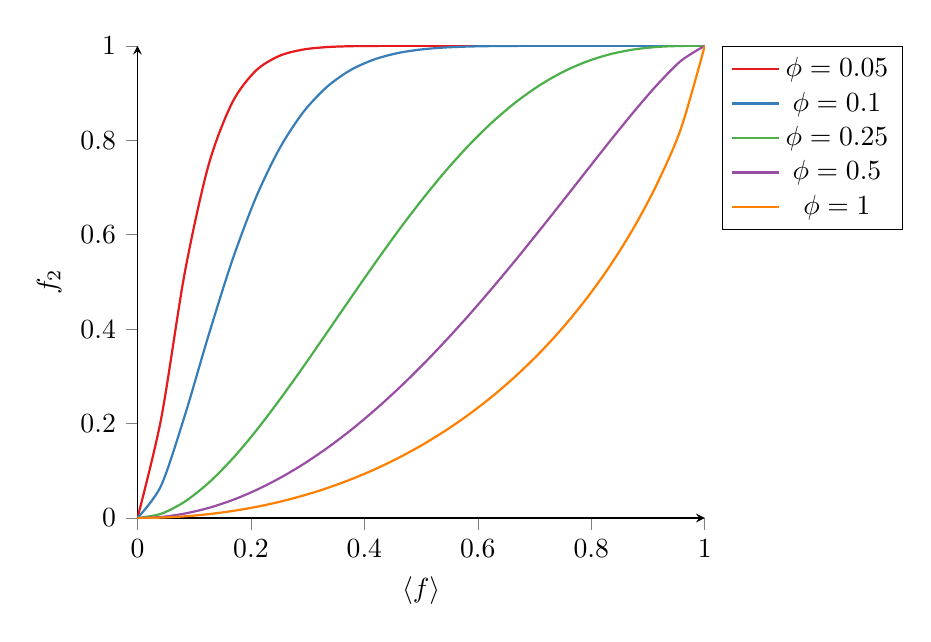
\begin{tikzpicture}[
		declare function={ f2app(\x,\y) = 1 - (1 - ln(1-\x) / \y) * (1-\x) ^ (1/\y);
		},
	]
	\begin{axis}[width=250pt,axis x line=bottom, axis y line=left, tick align=outside, domain=0:1, xmin=0, xmax=1, xlabel={$\fin$}, ylabel={$f_2$}, ymin=0, ymax=1, legend pos=outer north east]
	\addplot+[mark=none,smooth,thick] (\x,{ f2app(\x, 0.05) });
	\addlegendentry{$\phi = 0.05$}
	\addplot+[mark=none,smooth,thick] (\x,{ f2app(\x, 0.1) });
	\addlegendentry{$\phi = 0.1$}
	\addplot+[mark=none,smooth,thick] (\x,{ f2app(\x, 0.3) });
	\addlegendentry{$\phi = 0.25$}
	\addplot+[mark=none,smooth,thick] (\x,{ f2app(\x, 0.6) });
	\addlegendentry{$\phi = 0.5$}
	\addplot+[mark=none,smooth,thick] (\x,{ f2app(\x, 1) });
	\addlegendentry{$\phi = 1$}
	\end{axis}
	\end{tikzpicture}
\end{center}

Interestingly, we can reach the same solution by using the results from section \ref{sec:equal_taus}. First, since that solution contains $t/\tau$ also outside of the exponents, we need to find its expression as a function of $\fin$ explicitly:
\begin{eqnarray}
	\fin &=& 1 - e^{-\mu t} = 1 - e^{-\phi t / \tau} \\
	e^{-t/\tau} &=& (1 - \fin)^{1/\phi} \\
	t/\tau &=& -\ln{\left(1 - \fin\right)} / \phi
\end{eqnarray}
and if we insert these expressions into Equation \ref{eq:equal_tau_solution} for $i=2$, i.e. $f_2 = 1 - \left(1 + t/\tau \right) e^{-t/\tau}$, we see that it is identical to Equation \ref{eq:equal_phi_solution}.

\subsection{Observability of \texorpdfstring{$\phi_1$}{phi1} and \texorpdfstring{$\phi_2$}{phi2}}
It is noteworthy, that even though $f_2$ has two degrees of freedom ($\phi_1$ and $\phi_2$), the function is \textit{almost} redundant in parameter space, meaning that the shape of $f_2$ is almost constant if $\phi_1 \cdot \phi_2 = \text{const}$. Below is an example for a range of values, where $\phi_1 \cdot \phi_2 = 0.36$. We also compare that to the limit $\phi_1 = \phi_2 = 0.6$.

\begin{center}
	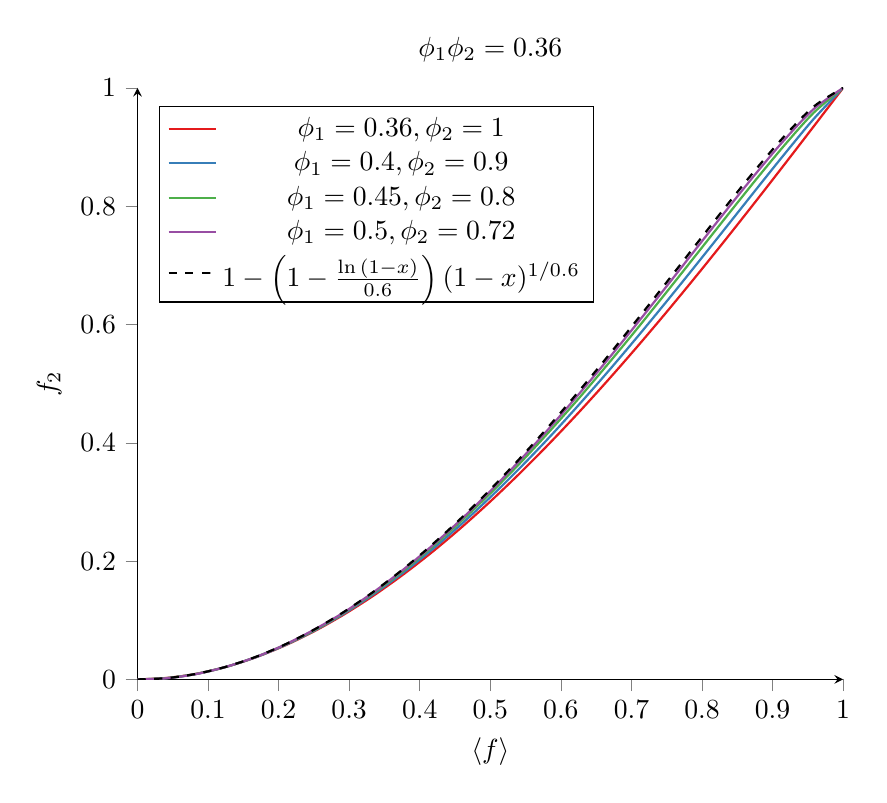
\begin{tikzpicture}[
	declare function={ f2(\x,\y,\z) = 1 + \y/(\z - \y)*(1-\x)^(1/\y) - \z/(\z - \y)*(1-\x)^(1/\z);
	},
	declare function={ f2app(\x,\y) = 1 - (1 - ln(1-\x) / \y) * (1-\x) ^ (1/\y);
	},
	]
	\begin{axis}[title={$\phi_1 \phi_2 = 0.36$}, width=300pt,axis x line=bottom, axis y line=left, tick align=outside, domain=0:1, xlabel={$\fin$}, ylabel={$f_2$}, ymin=0, ymax=1, legend pos=north west]
		\addplot+[mark=none,smooth,thick] (\x,{ f2(\x, 0.36, 1) });
		\addlegendentry{$\phi_1 = 0.36, \phi_2 = 1$}
		\addplot+[mark=none,smooth,thick] (\x,{ f2(\x, 0.4, 0.9) });
		\addlegendentry{$\phi_1 = 0.4, \phi_2 = 0.9$}
		\addplot+[mark=none,smooth,thick] (\x,{ f2(\x, 0.45, 0.8) });
		\addlegendentry{$\phi_1 = 0.45, \phi_2 = 0.8$}
		\addplot+[mark=none,smooth,thick] (\x,{ f2(\x, 0.5, 0.72) });
		\addlegendentry{$\phi_1 = 0.5, \phi_2 = 0.72$}
		\addplot+[color=black,dashed,mark=none,smooth,thick] (\x,{ f2app(\x, 0.6) });
		\addlegendentry{$1 - \left(1 - \frac{\ln{(1 - x)}}{0.6} \right) (1 - x)^{1/{0.6} }$}
	\end{axis}
	\end{tikzpicture}
\end{center}

This means, that if we try to fit these parameters to measured data, we might not be able to distinguish between a set of nearly equivalent solutions (with the same $\phi_1 \cdot \phi_2$ value).

\subsubsection{Example with pool size as parameters}
Given two scenarios, where the pool size ratios are 4:3:3 and 5:2:3, the $f_2$ trajectory will look exactly the same.

\begin{center}
	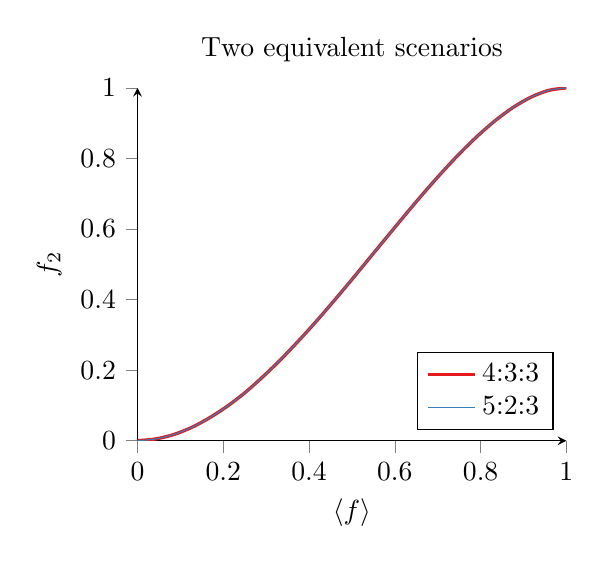
\begin{tikzpicture}[
	declare function={ f2(\x,\y,\z) = 1 + \y/(\z - \y)*(1-\x)^(1/\y) - \z/(\z - \y)*(1-\x)^(1/\z);
	},
	]
	\begin{axis}[title={Two equivalent scenarios}, width=200pt,axis x line=bottom, axis y line=left, tick align=outside, domain=0:1, xlabel={$\fin$}, ylabel={$f_2$}, ymin=0, ymax=1, legend pos=south east]
	\addplot+[mark=none,smooth,very thick] (\x,{ f2(\x, 0.4, 0.5) });
	\addlegendentry{4:3:3}
	\addplot+[mark=none,smooth] (\x,{ f2(\x, 0.5, 0.4) });
	\addlegendentry{5:2:3}
	\end{axis}
	\end{tikzpicture}
\end{center}

\section{Linear reversible pathway with dilution}
In this section, we relax our assumption that all reactions are irreversible, but keep focusing on linear pathways whose fluxes are determined by dilution. Unfortunately, the solution for general pathway lengths is extremely complex. Therefore, the only analytical solution we will discuss here is the case of $n = 2$.

\subsection{2-step assembly with reversibility}

\begin{equation}
    \overset{y}{\rightarrow} \underset{\downarrow}{S_1}
    \rightleftarrows \underset{\downarrow}{S_2}
\end{equation}
As before, we assume that the system is at balanced growth, so that the dilution fluxes are proportional to their pool sizes, i.e. $\mu s_i$. So:
\begin{eqnarray}
    y &=& \mu (s_1 + s_2)\\
    \flux{1}{2} &=& \mu s_2 + \flux{2}{1}
\end{eqnarray}

For simplicity, we define $x \equiv \flux{2}{1} / (\mu s_2)$, therefore:
\begin{align*}
    g_1 &= y/s_1 = \mu(1 + s_2/s_1)\\
    m_{11} &= -(\flux{2}{1} + y)/s_1 = -(\mu s_2 x + \mu s_1 + \mu s_2)/s_1 = 
    \mu ( -1 - (1 + x) s_2/s_1)\\
    m_{12} &= \flux{1}{2} / s_2 = (\mu s_2 + \mu s_2 x) / s_2 = 1 + x\\
    m_{21} &= \flux{2}{1} / s_1 = (\mu s_2 x) / s_1 = x s_2 / s_1\\
    m_{22} &= -(\flux{1}{2})/s_2 = -m_{12} = -1-x
\end{align*}

We can reduce the number of parameters further by setting $\phi \equiv \frac{s_1}{s_1+s_2}$:
\begin{eqnarray}
\mathbf{M} = \mu \cdot 
    \begin{bmatrix}
        - 1 - (1+x)(1/\phi-1) & 1+x \\
        x (1/\phi-1) & -1-x
    \end{bmatrix}
~~~~
\vec{g} = \mu \begin{bmatrix} 1/\phi & 0 & \ldots & 0 \end{bmatrix}
\end{eqnarray}
finding the Jordan normal form for $\mathbf{M}$ with \href{https://www.sympy.org/}{Sympy} and calculating:
\begin{eqnarray}
\vec{g}~\mathbf{P}~\mathbf{J}^{-1} = 
    \begin{bmatrix}
        -\frac{1}{1-\phi} & \frac{1}{x}
    \end{bmatrix}
~~~
e^{\mathbf{J} t} =
    \begin{bmatrix}
        e^{-\mu t} & 0 \\
        0 & e^{-\mu t (x+1)/\phi}
    \end{bmatrix}
~~~
\mathbf{P}^{-1} = 
    \begin{bmatrix}
		-\frac{x(\phi-1)}{x + 1 - \phi} & \frac{(1-\phi)(x+1)}{x + 1 - \phi} \\
		\frac{x(\phi-1)}{x + 1 - \phi} & \frac{\phi~x}{x + 1 - \phi} 
	\end{bmatrix}
\end{eqnarray}
which are combined to give the solution:
\begin{eqnarray}
    f(t) = 
    \vec{g} ~ \mathbf{P} ~ \mathbf{J}^{-1} ~ \left( e^{\mathbf{J t}} - \mathbf{I} \right) \mathbf{P}^{-1}
    = 
    \begin{bmatrix}
		\frac{1-e^{-\mu t}}{1-\phi} &
		-\frac{1 - e^{-\mu t (x+1)/\phi}}{x}
	\end{bmatrix}
    \begin{bmatrix}
		\frac{x(1-\phi)}{x + 1 - \phi} & \frac{(1-\phi)(x+1)}{x + 1 - \phi} \\
		-\frac{x(1-\phi)}{x + 1 - \phi} & \frac{\phi~x}{x + 1 - \phi} 
	\end{bmatrix}
\end{eqnarray}
If we focus only on $f_2(t)$:
\begin{eqnarray}
    f_2 &=& 
    \frac{x+1}{x+1-\phi} (1 - e^{-\mu t}) -
    \frac{\phi}{x+1-\phi}(1 - e^{-\mu t (x+1)/\phi})\\
    &=&
    1 - \frac{x+1}{x+1-\phi} e^{-\mu t} - 
    \frac{\phi}{x+1-\phi} e^{-\mu t (x+1)/\phi}
\end{eqnarray}
and make two substitutions: $\phi' \equiv \phi/(1+x)$ and $e^{-\mu t} = 1 - \fin$. Note that the derivation of $\fin$ in Equation \ref{eq:fin_dilution} is valid also in this system where internal fluxes are not irreversible, since it only depends on the exchange fluxes. Finally, we get:
\begin{eqnarray}
    f_2 ~=~ 
    1 + \frac{1}{1-\phi'} (1-\fin) + \frac{\phi'}{1-\phi'} (1-\fin)^{1/\phi'}
	\label{eq:two_step_reversible}\,.
\end{eqnarray}

Equation \ref{eq:two_step_reversible} is identical to the solution for $f_2$ in the 2-step irreversible model (Equation \ref{eq:two_step_f2_vs_ftot}), except that $\phi'$ replaces $\phi_1$. That means that for any $x > 0$, we will be able to fit $f_2$ as a function of $\fin$ precisely also with an irreversible model, and the precursor pool $\phi_1$ will be underestimated by a factor of $1+x$.

\subsection{Analytical solution for maturation time}
We define the maturation time $t_{1/2}$ as the time after which a protein that starts in $S_1$ to have a 50\% chance of reaching $S_2$. 

In the 2-step reversible model, the total flux from $S_1$ to $S_2$ is $\mu s_2 (1+x)$, and therefore the chance of any molecule in $S_1$ to make the transition in a short time interval $dt$ is $\mu s_2/s_1 (1+x) dt$. We can replace $s_2/s_1$ with $1/\phi_1 - 1$.

We denote by $P(t)$, the probability that our protein of interest has moved to $S_2$ (matured) before time $t$. The chance of making the transition exactly between $t$ and $t+dt$ is the probability it did not happen already before $t$ (which is $1 - P(t)$) times the probability we just calculated earlier:
\begin{eqnarray}
    dP &=& P(t + dt) - P(t) = \left(1 - P(t)\right) \mu s_2/s_1 (1+x) dt \\
    \int_0^T \frac{1}{1-P} dP &=& \int_0^T s_2/s_1 \mu (1+x)~dt  \\
    -\ln(1-P) &=& s_2/s_1 \mu (1+x)t = (1/\phi_1 - 1)\mu (1+x)t  \\
    t &=& \frac{-\ln(1-P(t))}{\mu (1+x)} \frac{\phi_1}{1 - \phi_1}\,.
\end{eqnarray}

Now, imagine that we fit the precursor pools using data while assuming that the reactions are irreversible. In this case, we are going to underestimate $\phi_1$ by a factor of $(1+x)$, when trying to estimate $t$. To understand how this assumption affects the result, we define our new estimate as:
\begin{eqnarray}
    t' &\equiv& \frac{-\ln(1-P)}{\mu} \cdot \frac{\phi'_1}{1 - \phi'_1} 
    = \frac{-\ln(1-P)}{\mu} \cdot \frac{\phi_1/(1+x)}{1 - \phi_1/(1+x)} \nonumber\\
    &=& \frac{-\ln(1-P)}{\mu (1+x)} \cdot \frac{\phi_1}{1 - \phi_1/(1+x)} 
    = t \cdot \frac{1 - \phi_1}{1 - \phi_1/(1+x)}
\end{eqnarray}
and therefore
\begin{eqnarray}
    1 ~\geq~ \frac{t'}{t} ~>~ 1-\phi_1
\end{eqnarray}
or in other words, if we use an irreversible model to find the maturation, we might underestimate it, but not by more than a factor of $1-\phi_1$.

\clearpage
\section{Fitting measured data}

\subsection{Using the 2-step model}
The common scenario would be that $\tau_i$ are unknown, and we have several time point measurements of some or all $f_i$. In this example, we assume again a 3-step chain, where we measure $\fin$ and $f_2$, and the free parameters are $\phi_1$ and $\phi_2$. 

\subsection{How to infer fluxes from labeling data}

We assume that the data was generated from a system such as in equation \ref{eq:inhom_ode}, with a diagonalizable matrix $\mathbf{M}$. Then, we can fit our data (which is $\vec{f}$ measured at multiple time points) using the formula $\vec{f}(t) = \mathbf{A} e^{\vec{\lambda} t}$. Then, from equation \ref{eq:inhom_ode_sol} we know that $\mathbf{P} = \mathbf{A} \mathbf{D}^{-1}$, where $\mathbf{D}$ is some fully ranked diagonal matrix. Even though $\mathbf{D}$ is somehow dependent on $\mathbf{P}$ and $\mathbf{A}$, it wouldn't matter for finding $\mathbf{M}$, since:
\begin{eqnarray}
    \mathbf{M} = \mathbf{P}~\text{diag}(\vec{\lambda})~\mathbf{P}^{-1} = \mathbf{A}\mathbf{D}^{-1}~\text{diag}(\vec{\lambda})~\mathbf{D}\mathbf{A}^{-1} = 
    \mathbf{A}\mathbf{D}^{-1}\mathbf{D}~\text{diag}(\vec{\lambda})~\mathbf{A}^{-1} = 
    \mathbf{A}~\text{diag}(\vec{\lambda})~\mathbf{A}^{-1}
\end{eqnarray}
where $\text{diag}(\vec{\lambda})~\mathbf{D} = \mathbf{D}~\text{diag}(\vec{\lambda})$ since they are both diagonal matrices. Therefore, we can simply ignore the $\mathbf{D}$ matrix altogether, and use the solution:
\begin{eqnarray}
    \mathbf{\bar{V}} = \mathbf{M}^\top~\text{diag}(\vec{s}) = \left(\mathbf{A}~\text{diag}(\vec{\lambda})~\mathbf{A}^{-1} \right)^\top~\text{diag}(\vec{s})
\end{eqnarray}
where $\mathbf{\bar{V}} = \mathbf{V} - \text{diag}(\vec{1}_n~\mathbf{V})$, i.e. the fluxes would be the off-diagonal values of $\mathbf{\bar{V}}$.

\section{Layers}
What if $\vec{g}(t)$ is not constant. If we know that it is itself generated by a (in)homogeneous linear ODE system, we can safely assume it can be described by a series of exponents:
\begin{eqnarray}
    \vec{g}(t) = \vec{\alpha} e^{\mathbf{G} t} + \vec{\beta}
\end{eqnarray}
for some $\vec{\beta} \in \mathbb{R}^n$ and $\mathbf{G} \in \mathbb{R}^{n \times n}$. Note that we can use zero padding ensure that the size of $\vec{\beta}$ and $\mathbf{G}$ match the number of internal pools. Now, we can solve Equation \ref{eq:inhom_ode_sol} for cases where $\vec{g}$ is not constant:
\begin{eqnarray}
    \vec{f}(t) &=&
    \vec{f}(0)~e^{\mathbf{M} t} ~+~ \int_0^t \left(\vec{\alpha} e^{\mathbf{G} \tau} + \vec{\beta}\right) e^{\mathbf{M} (t-\tau)} d\tau \nonumber\\
    &=&
    \vec{f}(0)~e^{\mathbf{M} t} ~+~ \left[
    \vec{\alpha} \int_0^t e^{(\mathbf{G} - \mathbf{M})\tau} d\tau ~+~ 
    \vec{\beta} \int_0^t e^{-\mathbf{M}\tau} d\tau 
    \right] e^{\mathbf{M} t} \nonumber\\
    &=& 
    \vec{f}(0)~e^{\mathbf{M} t} ~+~ \left[
    \vec{\alpha}~(\mathbf{G}-\mathbf{M})^{-1}~(e^{(\mathbf{G} - \mathbf{M})t} - \mathbf{I}) ~-~ 
    \vec{\beta}~\mathbf{M}^{-1}~(e^{-\mathbf{M}t} - \mathbf{I})
    \right] e^{\mathbf{M} t} \nonumber\\
    &=&
    \vec{f}(0)~e^{\mathbf{M} t} ~+~
    \vec{\alpha}~(\mathbf{G}-\mathbf{M})^{-1}~(e^{\mathbf{G}t} - e^{\mathbf{M}t}) ~+~ 
    \vec{\beta}~\mathbf{M}^{-1}~(e^{\mathbf{M} t} - \mathbf{I})
    \label{eq:non_constant_g}
\end{eqnarray}
where we can see that the time independent part ($\vec{\beta}$) is the same as in our previous solution.

Therefore, if we separate the ODE system into layers where information only flows from top layers to lower ones, we can iteratively solve the ODE system in smaller chunks, rather then all at once. This could significantly accelerate the computation time \cite{young_elementary_2008}.

\subsection{Example: 2-step irreversible pathway}
Just to demonstrate how the layers work, we focus again on the 2-step irreversible pathway. We will start by using the solution for the first pool which is $h_1(t) = 1 - e^{-t/\tau_1}$ and show how we can use Equation \ref{eq:non_constant_g} to solve $f_2(t)$.

We start by describing the exchange function:
\begin{eqnarray}
    \vec{g}(t) = h_1(t) \frac{v_{1 \rightarrow 2}}{s_2} = (1 - e^{-t/\tau_1}) \frac{1}{\tau_2}
\end{eqnarray}
which means that $\vec{\alpha} = [-1/\tau_2]$, $\beta = [1/\tau_2]$ and $\mathbf{G} = [-1/\tau_1]$. The internal matrix is given by $\mathbf{M} = [-1/\tau_2]$. Using these values in Equation \ref{eq:non_constant_g} we get:
\begin{eqnarray}
    \vec{f}(t) &=& (-1/\tau_2) (-1/\tau_1 + 1/\tau_2)^{-1} (e^{-t/\tau_1} - e^{-t/\tau_2}) + (1/\tau_2) (-1/\tau_2)^{-1} (e^{-t/\tau_2} - 1) \nonumber\\
    &=& \frac{-\tau_1}{\tau_1 - \tau_2} (e^{-t/\tau_1} - e^{-t/\tau_2}) - (e^{-t/\tau_2} - 1)
    = 1 - \frac{\tau_1}{\tau_1 - \tau_2} e^{-t/\tau_1} + \frac{\tau_2}{\tau_1 - \tau_2} e^{-t/\tau_2}
\end{eqnarray}
which is the same solution as we get by solving $f_1$ and $f_2$ together.

\bibliographystyle{unsrt}
\bibliography{references}

\end{document}